% Number 870
% CAPMG Units 
% Car skidding to a stop graphical
% JG

% Watermark
\AddToShipoutPicture*{\BackgroundPic}

\addtocounter {ProbNum} {1}

%\begin{floatingfigure}[r]{.44\textwidth}
%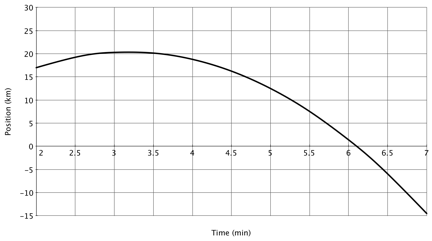
\includegraphics[scale=.5]{/Users/jgates/desktop/latex/pics/xgraph2}
%\end{floatingfigure}
 
{\bf \Large{\arabic{ProbNum}}} A car traveling with a speed of 30 meters per second (a little more than 60 mph) slams on the brakes.  The wheels lock up and the tires skid on the road, providing an acceleration of magnitude ${11~\tfrac{m}{s^2}}$.   \bigskip

How far did the car travel during the slide? Use graphical methods.\paragraph{}
\noindent
\vfill


%\begin{center}
%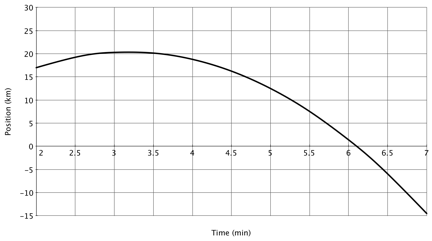
\includegraphics[scale=1]{/Users/jgates/desktop/latex/pics/xgraph2}
%\end{center}


\newpage